\documentclass[dvips, intlimits, 9pt, unicode, notheorems, color=usenames,dvipsnames]{beamer}
\usepackage{beamerthemesplit}
\usepackage[english, russian]{babel}
\usepackage[utf8x]{inputenc}
\usepackage[T1,T2A]{fontenc}
\usepackage{amsthm}
\usepackage{amsmath}
\usepackage{amssymb}
\usepackage{float}
\usepackage{graphicx}
\usepackage{algorithm}
\usepackage{algorithmic}
\usepackage{color}
\usepackage{array}
\usepackage{ulem}

\graphicspath{{../figures/eps/color/}}

\def\figureref#1{Рис.\,\protect\ref{#1}}
\def\eqref#1{(\protect\ref{#1}\protect)}

\floatname{algorithm}{Алгоритм}
\theoremstyle{plain}
\newtheorem{theorem}{Теорема}
\newtheorem{lemma}{Лемма}
\theoremstyle{definition}
\newtheorem{definition}{Определение}

\usetheme{Warsaw}
\usecolortheme{albatross}

\definecolor{pagecolor}{rgb}{0.16,0.208,0.318}
%\definecolor{btext}{rgb}{0.68,0.790,1}
%\definecolor{ytext}{rgb}{0.973,0.808,0.587}
%\definecolor{otext}{rgb}{1.0,0.6,0.306}
\beamersetaveragebackground{pagecolor}

\def\putReid#1{\raise-4mm\hbox{\protect\includegraphics[origin=c]{reidemeister-#1.eps}}}
\def\putSk#1{\raise-3.5mm\hbox{\protect\includegraphics[origin=c, scale=0.7]{tangle-jones-skein-example-#1.eps}}}
\def\putGen#1{\raise-5mm\hbox{\includegraphics[origin=c, scale=0.7]{border-deletion-sequence-#1.eps}}}

\title{ Классификация танглов }
\author{ В.~Р.~Мешков, А.~С.~Мишунин, А.~В.~Омельченко}
\date{ 15 июня 2011 г. }

\begin{document}
	\Russian

	\begin{frame}
		\maketitle
	\end{frame}

	\begin{frame}
		\frametitle{Теория узлов}

		Узел --- гладкое вложение $S^1$ в $\mathbb{R}^3$. Зацепление --- гладкое вложение набора из конечного числа $S^1$ в $\mathbb{R}^3$.

		\begin{figure}[ht]
			\centering
			\includegraphics[scale = 0.5]{c/knot-table.eps}
		\end{figure}

		Узлы можно перечислять, оперируя их плоскими диаграммами. При этом диаграммы соответствуют одному и тому же узлу тогда и только тогда,
		когда одну из них можно получить из другой при помощи движений Рейдемейстера:

		$$
			\putReid{11}\ \backsimeq\ \putReid{12},\qquad
			\putReid{21}\ \backsimeq\ \putReid{22},\qquad
			\putReid{31}\ \backsimeq\ \putReid{32}.
		$$
	\end{frame}

	\begin{frame}
		\frametitle{Виртуальные узлы}

		Пусть $S$ --- замкнутая двумерная ориентируемая поверхность рода $g > 0$. Тогда можно рассмотреть узлы и зацепления в $S \times \mathbb{R}$,
		называемые виртуальными.
		\begin{figure}[ht]
			\centering
			\includegraphics[scale = 0.5]{c/genus-2-link.eps}
		\end{figure}

		Существует возможность разделить виртуальное зацепление на две части, отвечающие за <<перекрестки>> и за <<поверхность>> соответственно:
		\begin{figure}[ht]
			\centering
			\includegraphics[scale = 0.5]{c/tangle-star-example.eps}
		\end{figure}
	\end{frame}

	\begin{frame}
		\frametitle{Танглы}

		На виртуальных узлах можно определить операцию стягивания:
		\begin{figure}[ht]
			\centering
			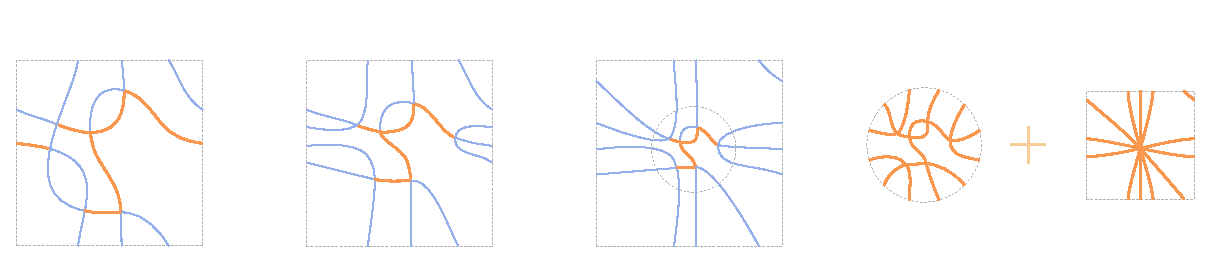
\includegraphics[scale = 0.4]{c/virtual-contraction.eps}
		\end{figure}

		\begin{definition}
			\label{definition:tangle}
			$k$-танглом называется гладкое вложение $k$ отрезков и конечного числа окружностей в $B^3$
			(трехмерный замкнутый шар единичного радиуса), если $2k$ концов отрезков взаимно однозначно отображаются
			на точки с координатами $(\cos\pi i/k, \sin\pi i/k, 0)$, $i\in\{0, 1, \dots, 2k{-}1\}$, называемые
			концами $k$-тангла, и больше ни какие точки отрезков или окружностей на границу $B^3$ не отображаются.
		\end{definition}

		\begin{figure}[ht]
			\centering
			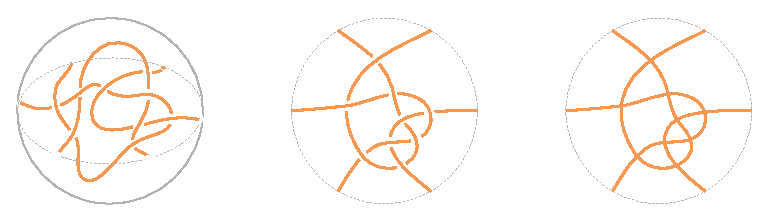
\includegraphics[scale = 0.6]{c/tangle-diagram-projection.eps}
		\end{figure}
	\end{frame}

	\begin{frame}
		\frametitle{Требования к рассматриваемым проекциям}

		Первой нашей задачей будет перечислеие проекций. При этом мы наложим на множество рассматриваемых проекций
		несколько естественных ограничений:
		\begin{itemize}
			\item Мы не будем различать проекции, отличающиеся только гомеоморфизмом (поворотом, отражением).
			\item Мы будем рассматривать только простые проекции.
			\item Мы будем рассматривать только связные проекции. В противном случае число проекций для любого фиксированного
			количества перекрестков будет бесконечным.
		\end{itemize}

		\begin{figure}
			\centering
			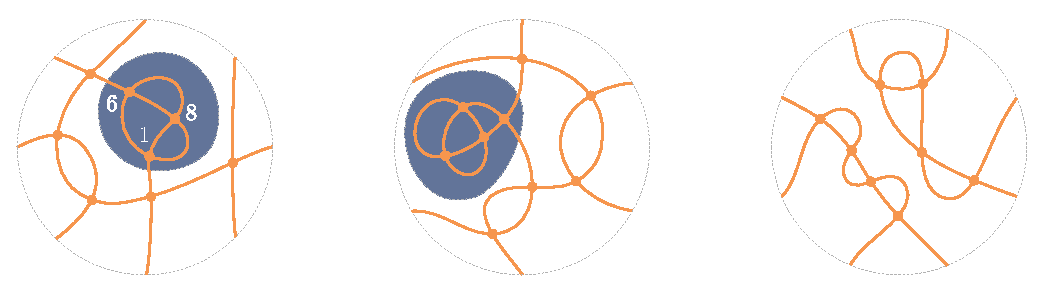
\includegraphics[scale = 0.5]{c/composite-non-connected-projections.eps}
		\end{figure}

		Диаграмма (проекция) $k$-тангла называется составной, если существует замкнутая несамопересекающаяся кривая, которая трансверсально
		пересекает диаграмму ровно в двух точках и содержит внутри как минимум один перекресток. В противном случае диаграмма называется простой.
	\end{frame}

	\begin{frame}
		\frametitle{Операции с проекциями}

		\begin{figure}[ht]
			\centering
			$\putGen{6} {}\to{} \putGen{5} {}\to{} \putGen{4} {}\to{} \putGen{3} {}\to{} \putGen{2} {}\to{} \putGen{1}$
		\end{figure}

		\begin{theorem}
			В любой связной простой проекции $k$-тангла, содержащей более одного перекрестка, можно удалить пограничный
			перекресток так, чтобы получившаяся в результате проекция была простой и связной.
		\end{theorem}
	\end{frame}

	\begin{frame}
		\frametitle{Точки сочленения}

		Простота любой получающейся проекции очевидна. Осталось доказать возможность получения связной проекции, показав,
		что среди пограничных перекрестков найдется не являющийся точкой сочленения проекции. Точка сочленения --- перекресток,
		через которую можно провести хорду (гладкую несамопересекающуюся кривую, только начало и конец которой лежат на граничной
		окружности), которая больше нигде с проекцией не пересекается, и с обеих сторон от которой есть перекрестки.
		\begin{figure}[ht]
			\centering
			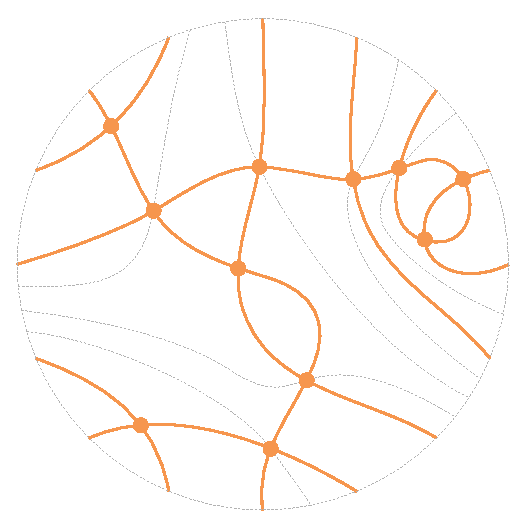
\includegraphics[scale = 0.5]{c/cutpoints-proof.eps}
		\end{figure}
	\end{frame}

	\begin{frame}
		\frametitle{root-code}

		root-code$(P, v) = \min_{e \in v, f \in \{CW, CCW\} } $root-code$(P, v, e, f)$

		\begin{block}{root-code$(P, (v, e, f))$}
		{
			\footnotesize
			\begin{algorithmic}[H]
				\STATE $A \leftarrow \{\}$
				\STATE $free \leftarrow 2$

				\STATE $Q \leftarrow \{v\}$
				\STATE $number[v] \leftarrow 1$
				\STATE $incoming[v] \leftarrow e$

				\WHILE{$Q \neq \varnothing$}
					\STATE $u \leftarrow head[Q]$
					\STATE $dequeue(Q)$

					\FOR{(для) всех ребер $(u, w) \in P$ в порядке, заданном $f$, начиная с $incoming[u]$}
						\IF{$w$ --- конец диаграммы}
							\STATE $code \leftarrow 0$
						\ELSE
							\IF{$number[w]$ не определен}
								\STATE $number[w] \leftarrow free$
								\STATE $free \leftarrow free + 1$
								\STATE $enqueue(Q, w)$
							\ENDIF
							\STATE $code \leftarrow number[w]$
						\ENDIF

						\STATE $push(A, code)$
					\ENDFOR
				\ENDWHILE

				\RETURN $A$
			\end{algorithmic}
		}
		\end{block}
	\end{frame}

	\begin{frame}
		\frametitle{Примеры root-code}

		\begin{figure}[ht]
			\centering
			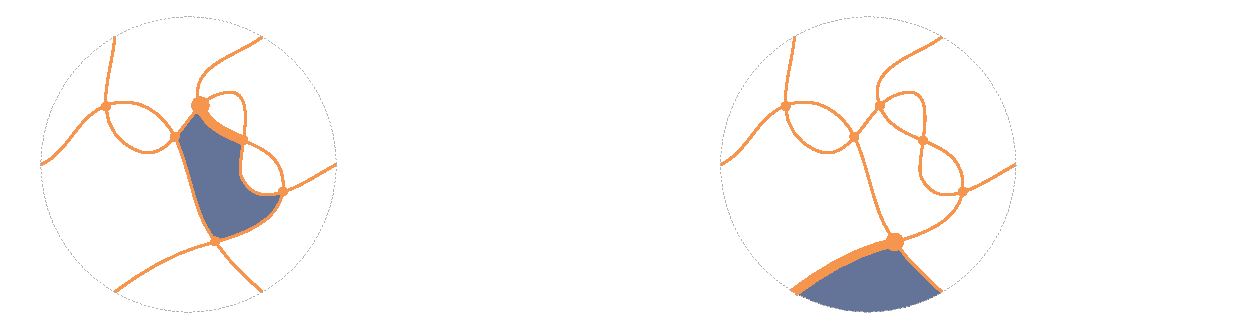
\includegraphics[scale = 0.5]{c/rcode-example.eps}
		\end{figure}
	\end{frame}

	\begin{frame}
		\frametitle{Дерево проекций}

		\begin{definition}
			Пусть $I$ --- проекция тангла, состоящая из единственного пререкрестка. Определим на множестве простых связных
			проекций $k$-танглов отображение $prev(T)$ следующим образом:
			\begin{itemize}
				\item
				$prev(I) = \varnothing$

				\item
				Для всех остальных $prev(T)$ будет являться результатом удаления из $T$ пограничного перекрестка $v$, не
				являющегося точкой сочленения, такого что root-code($T$, $v$) лексикографически минимален среди всех подобных
				перекрестков.
			\end{itemize}
		\end{definition}

		\begin{itemize}
			\item $prev(T)$ определено на всем множестве простых связных проекций $k$-танглов.
			\item $prev(T)$ однозначно относительно гомеоморфизмов.
			\item $prev(T)$ всегда уменьшает полуинвариант --- число перекрестков.
		\end{itemize}
	\end{frame}

	\begin{frame}
		\frametitle{Дерево проекций}

		\begin{figure}[ht]
			\centering
			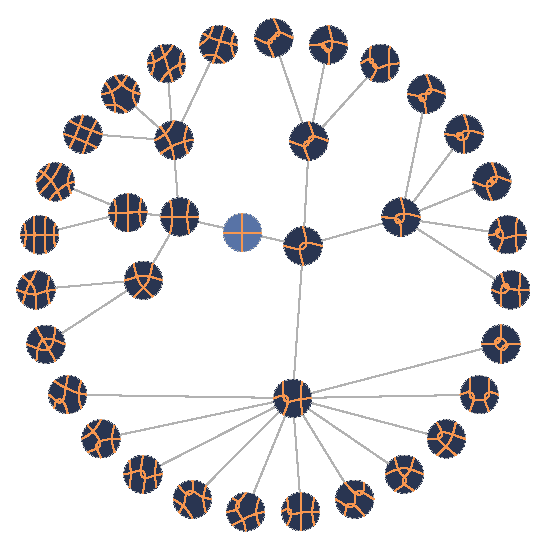
\includegraphics[scale = 0.9]{c/genealogical-tree.eps}
		\end{figure}
	\end{frame}

	\begin{frame}
		\frametitle{Алоритм}

		Основная идея --- обход полученного дерева в глубину.
		\begin{block}{DFS(T)}
		{
			\footnotesize
			\begin{algorithmic}[H]
				\algsetup{linenosize=\small, linenodelimiter=.}
				\PRINT $T$
				\IF{$crossings(T) = n$}
					\RETURN
				\ENDIF

				\STATE $list \leftarrow \varnothing$
				\FOR{(для) всех возможных результатов $R$ приклеивания перекрестка $v$ к $T$}
					\IF{$R$ --- простая}
						\IF{$prev(R) = T$}
							\STATE $r \leftarrow $ root-code($R$, $v$)
							\IF{ {\bf not} $contains(list, r)$}
								\STATE DFS($R$)
								\STATE $add(list, r)$
							\ENDIF
						\ENDIF
					\ENDIF
				\ENDFOR
			\end{algorithmic}
		}
		\end{block}

		Преимущества подхода:
		\begin{itemize}
			\item Не нужна хеш-таблица.
			\item Легко распараллелить.
			\item Легко обобщить.
		\end{itemize}
	\end{frame}


	\begin{frame}
		\frametitle{Альтернированные танглы}

		\begin{definition}
			Альтернированной диаграммой называется та, у которой любая нить, соединяющее два перекрестка, в одном из них проходит
			сверху, а в другом --- снизу. Альтернированный тангл --- тангл, имеющий альтернированную диаграмму.
		\end{definition}

		\begin{itemize}
			\item Любая простая альтернированная диаграмма является минимальной по числу перекрестков.
			\item (Tait flyping conjecture) Все минимальные диаграммы простого альтернированного тангла могут быть
			получены друг из друга применением преобразования, называемого “flype”:
		\end{itemize}

		\begin{figure}[ht]
			\centering
			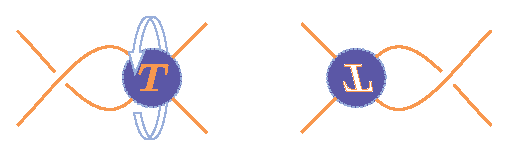
\includegraphics[scale = 1]{c/flype.eps}
		\end{figure}
	\end{frame}

	\begin{frame}
		\frametitle{Теорема о пересекающихся танглах}

		Под словом <<тангл>> ниже будет подразумеваться простая связная диаграмма альтернированного $2$-тангла.

		\begin{theorem}
			\label{theorem:tangle-decomp-th}
			Пусть у нас есть два связных тангла $A$ и $B$, содержащиеся в какой-то простой альтернированной диаграмме
			тангла или зацепления $D$. При этом $A\setminus B\neq\varnothing$, $B\setminus A\neq\varnothing$
			и $A\cap B\neq\varnothing$. Тогда $A\setminus B$, $B\setminus A$, $A\cap B$ и $A\cup B$ --- также связные
			танглы, а $A\cup B$ представим в виде:

			\begin{figure}[H]
				\centering
				\includegraphics{tangle-decomp-theorem.eps}
			\end{figure}
		\end{theorem}
	\end{frame}

	\begin{frame}
		\frametitle{Идея доказательства}

		\begin{figure}[H]
			\centering
			\includegraphics[scale = 0.8]{tangle-decomp-proof.eps}
		\end{figure}

		\begin{equation}
			\label{equation:a_relation}
			a + c + e + f = 4
		\end{equation}
		\begin{equation}
			\label{equation:b_relation}
			b + c + d + f = 4
		\end{equation}

		\begin{equation}
			\label{equation:ab_relation}
			d + e + c \ge 4
		\end{equation}
		\begin{equation}
			\label{equation:all_relation}
			a + b + c \ge 4
		\end{equation}
		\begin{equation}
			\label{equation:amb_relation}
			a + d + f \ge 4
		\end{equation}
		\begin{equation}
			\label{equation:bma_relation}
			b + e + f \ge 4
		\end{equation}
	\end{frame}

	\begin{frame}
		\frametitle{$2$-тангл структура}

		Требования к разложению $v \in T \rightarrow S(v) \subset T$:
		\begin{itemize}
			\item $v \in S(v)$
			\item $\forall R \subset T$, где $R$ --- $2$-тангл, $v \in R \Rightarrow R \subset S(v)$
			\item $\forall u, u \in S(v) \Leftrightarrow S(u) = S(v)$
		\end{itemize}

		\begin{figure}[ht]
			\centering
			\includegraphics[scale = 0.8]{tangle-decomp-example.eps}
		\end{figure}

		Для $2$-танглов, в свою очередь, можно определить правила <<сборки>> из $2$-танглов меньшего
		размера. При этом $2$-танглы, представимые в виде прямой суммы, рассматриваются отдельно.

		\begin{figure}[H]
			\centering
			\includegraphics[scale = 0.5]{tangle-sum.eps}
		\end{figure}
	\end{frame}

	\begin{frame}
		\frametitle{Обобщение root-code}

		\begin{block}{root-code$(P, (v, e, f))$}
		{
			\footnotesize
			\begin{algorithmic}[H]
				\STATE $A \leftarrow \{\}$
				\STATE $free \leftarrow 2$

				\STATE $Q \leftarrow \{v\}$
				\STATE $number[v] \leftarrow 1$
				\STATE $incoming[v] \leftarrow e$

				\WHILE{$Q \neq \varnothing$}
					\STATE $u \leftarrow head[Q]$
					\STATE $dequeue(Q)$

					\STATE \textcolor{red}{$push(A, tangle(u))$}

					\FOR{(для) всех ребер $(u, w) \in P$ в порядке, заданном $f$, начиная с $incoming[u]$}
						\IF{$w$ --- конец диаграммы}
							\STATE $code \leftarrow 0$
						\ELSE
							\IF{$number[w]$ не определен}
								\STATE $number[w] \leftarrow free$
								\STATE $free \leftarrow free + 1$
								\STATE $enqueue(Q, w)$
							\ENDIF
							\STATE $code \leftarrow number[w]$
						\ENDIF

						\STATE $push(A, code)$
					\ENDFOR

					\STATE \textcolor{red}{$push(A, orientation(u, incoming[u], f))$}
				\ENDWHILE

				\RETURN $A$
			\end{algorithmic}
		}
		\end{block}
	\end{frame}

	\begin{frame}
		\frametitle{$2$-танглы}

		В любой прямой сумме можно (и нужно) перегнать все одиночне перекрестки на одну из двух сторон с помощью флипов:
		\begin{figure}[ht]
			\centering
			\includegraphics[scale = 0.5]{one-side-crossings.eps}
		\end{figure}

		\vspace{-6mm}
		\begin{table}[ht]
			\caption{Правила сборки прямых сумм\label{table:sums-rules}}
			\centering
			\begin{tabular}{cm{22mm}l}
				\hline
				1 & \includegraphics[scale = 0.5]{alternating-build-4-case-1.eps} & --- принять \\
				2 & \includegraphics[scale = 0.5]{alternating-build-4-case-2.eps} & --- принять \\
				3 & \includegraphics[scale = 0.5]{alternating-build-4-case-3.eps} & --- сравнить по root-code \\
				4 & \includegraphics[scale = 0.5]{alternating-build-4-case-4.eps} & --- нарушается положение перекрестков \\
				5 & \includegraphics[scale = 0.5]{alternating-build-4-case-5.eps} & --- нарушается положение перекрестков \\
				6 & \includegraphics[scale = 0.5]{alternating-build-4-case-6.eps} & --- не бывает \\
				7 & \includegraphics[scale = 0.5]{alternating-build-4-case-7.eps} & --- принять \\
				8 & \includegraphics[scale = 0.5]{alternating-build-4-case-8.eps} & --- не бывает \\
				\hline
			\end{tabular}
		\end{table}

		\begin{center}
			{\bf У одиночного перекрестка должен быть минимальный номер.}
		\end{center}
	\end{frame}

	\begin{frame}
		\frametitle{Альтернированные танглы: результаты}

		\begin{figure}[H]
			\centering
			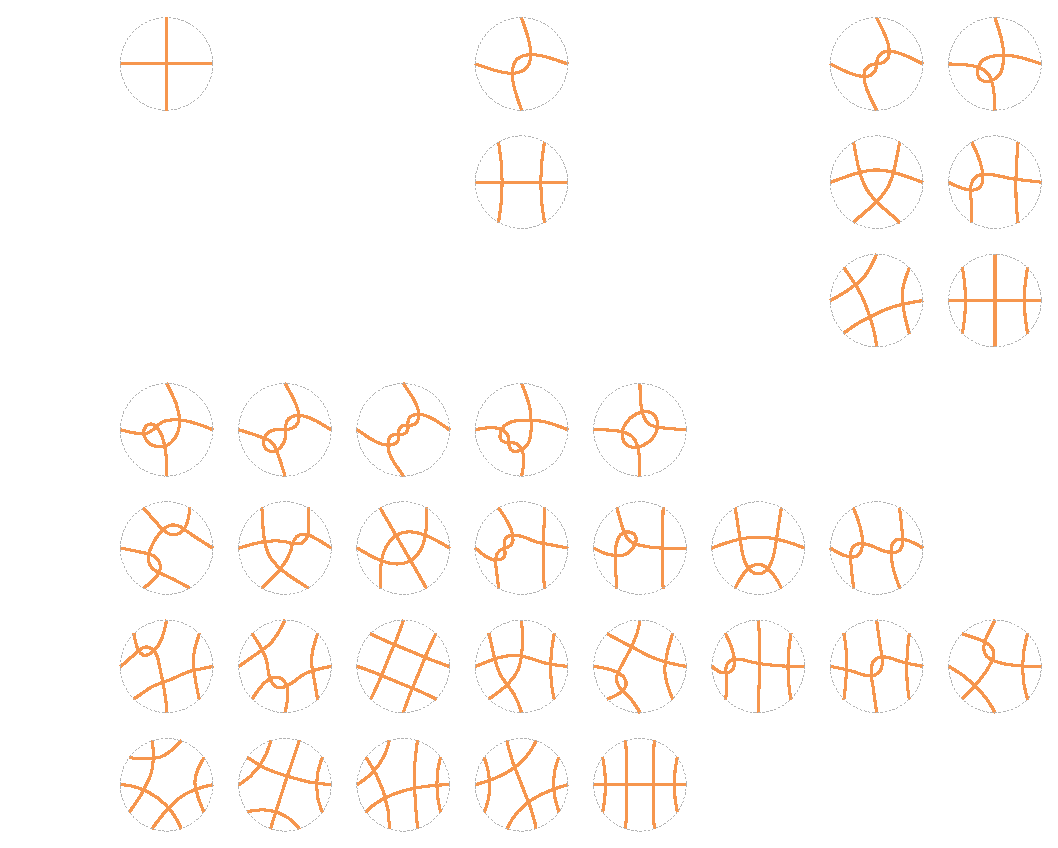
\includegraphics[scale = 0.5]{c/alternating-tangles-1-4.eps}
		\end{figure}
	\end{frame}

	\begin{frame}
		\frametitle{Альтернированные танглы: результаты}

		\begin{table}[ht]
		{
			\tiny
			\caption{Количество альтернированных $k$-танглов с $n$ перекрестками.\label{table:alternating-tangles-table}}
			\centering
			\begin{tabular}{|c||r|r|r|r|r|r|r|r|r|r|r|r|}
			\hline
			$k$\textbackslash $n$
			    &               1 &               2 &               3 &               4 &                5 &                 6 &                    7 &                    8 &                     9 &                    10 &                     11 \\
			\hline\hline
			2   & \color{Gray}{1} & \color{Gray}{1} & \color{Gray}{2} & \color{Gray}{5} & \color{Gray}{13} & \color{Gray}{ 36} &    \color{Gray}{111} &    \color{Gray}{373} &  \color{Gray}{1\,362} &  \color{Gray}{5\,378} &  \color{Gray}{22\,807} \\
			3   &               . & \color{Gray}{1} & \color{Gray}{2} & \color{Gray}{7} & \color{Gray}{20} & \color{Gray}{ 77} &    \color{Gray}{276} & \color{Gray}{1\,135} &  \color{Gray}{4\,823} & \color{Gray}{21\,734} &               101\,307 \\
			4   &               . &               . & \color{Gray}{2} & \color{Gray}{8} & \color{Gray}{37} & \color{Gray}{157} &    \color{Gray}{687} & \color{Gray}{3\,052} & \color{Gray}{13\,981} &               65\,797 &               317\,506 \\
			5   &               . &               . &               . & \color{Gray}{5} & \color{Gray}{31} & \color{Gray}{209} & \color{Gray}{1\,128} & \color{Gray}{5\,986} &               30\,556 &              155\,964 &               795\,918 \\
			6   &               . &               . &               . &               . & \color{Gray}{16} & \color{Gray}{161} & \color{Gray}{1\,294} &                \,528 &               51\,475 &              294\,366 &            1\,637\,855 \\
			7   &               . &               . &               . &               . &                . & \color{Gray}{ 60} &                  840 &               8\,206 &               62\,895 &              428\,254 &            2\,702\,902 \\
			8   &               . &               . &               . &               . &                . &                 . &                  261 &               4\,702 &               52\,815 &              460\,189 &            3\,475\,551 \\
			9   &               . &               . &               . &               . &                . &                 . &                    . &               1\,243 &               26\,753 &              341\,878 &            3\,327\,424 \\
			10  &               . &               . &               . &               . &                . &                 . &                    . &                    . &                6\,257 &              155\,593 &            2\,221\,544 \\
			11  &               . &               . &               . &               . &                . &                 . &                    . &                    . &                     . &               32\,721 &               916\,595 \\
			12  &               . &               . &               . &               . &                . &                 . &                    . &                    . &                     . &                     . &               175\,760 \\
			13  &               . &               . &               . &               . &                . &                 . &                    . &                    . &                     . &                     . &                      . \\
			\hline
			все &               1 &               2 &               6 &              25 &              117 &               700 &               4\,597 &              33\,225 &              250\,917 &           1\,961\,874 &           15\,695\,169 \\
			\hline
			\end{tabular}
		}
		\end{table}

		Хранения в памяти требуют только помеченные серым танглы.
	\end{frame}


	\begin{frame}
		\frametitle{Полиномиальный инвариант танглов}

		Пусть диаграммы $\ell$, $\ell_1$ и $\ell_2$ совпадают за пределами маленького круга, а внутри него выглядят следующим образом: 
		\begin{figure}[ht]
			\centering
			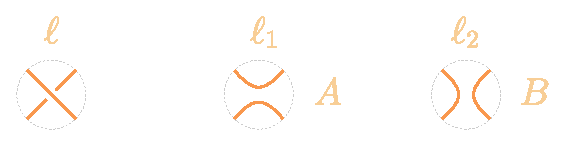
\includegraphics[scale = 0.6]{c/kauffman-skein-definition.eps}
		\end{figure}

		Определим для диаграммы полином по следующим правилам:
		$$
		\begin{aligned}
			& \langle \ell \rangle = a\langle \ell_1 \rangle + \frac{1}{a} \langle {\ell_2} \rangle \\
			& \langle {\ell{\textstyle{}\bigcup{}}\bigcirc} \rangle = -(a^2 + \frac{1}{a^2}) \langle \ell \rangle \\
		\end{aligned}
		$$

		В случае обычных узлов и зацеплений добавляется соотношение $\langle \bigcirc \rangle = 1$, однако для танглов конечными результатами
		расщеплений будут диаграммы без перекрестков. Возьмем здесь в качестве терминальных значений элементы модуля с базисом из таких диаграмм:

		\begin{figure}[ht]
			\centering
			$\putSk{1} = a^3 \putSk{2} + a \putSk{3} + (a - a^{-3}) \putSk{4} + (a^{-1} - a^{-5}) \putSk{5}$
		\end{figure}

		Полученный полином позволяет получить топологический инвариант танглов --- аналог полинома Джонса.
	\end{frame}
\end{document}
